% !Mode\dots ``TeX:UTF-8''
% !TEX root = ../bare_jrnl.tex
\section{The online observability of \BCNs}
\label{sec:online}


In this section we propose the online observability to solve the problem mentioned before, and we will introduce its related information in detail. 
%\begin{definition}
	 %In the online observability we determine the state of \BCN\ by observing its output sequence and then deriving and deciding the input sequence at every time step. What is more, this process can be accomplished in finite time steps.
%\end{definition}  without presupposing the initial state of \BCN





\ly{In the existing third and fourth observability, there has to exist an input sequence that determines its initial state $s_0$ if a \BCN\ satisfies the observability. }
But we can derive the set of possible initial states $\mathsf{S}(0)$ by initial output $\mathsf{o}(0)$ we observe at time step $0$, and then we find input sequence to determine initial state ($s_0\in S_0$) for different sets of possible initial states. These input sequences can be different, and we can also determine the initial state of the \BCN.
In this case, the requirements for the \BCN\ to determine the initial state would be less harsh since we utilize the set of possible initial states $S_0$ to find the input sequence. Furthermore, if we utilize the sets of possible initial states $S_0$ and $S_1$ derived in time step $0$ and $1$ to find the input sequence to determine the initial state, the requirements for \BCNs\ would further less harsh. 

According to this law, in the online observability we find input sequence by the $S_t$ we derive at every time step, such that the requirements would be least harsh. Thus, a \BCN\ satisfies the online observability iff its initial state $s_0$ can be determined in real time for every $s_0 \in \Delta_N$.

\tl{do not understand this at all, what does it mean by harsh?}

The reason why we called this type of observability online observability is as follows.
\begin{itemize}
  \item Firstly, in the online observability, we determine the initial state of \BCNs\ in real time. In other words, we only need one test case to determine the initial state of \BCNs. We call this property {\em real-time} property.%Such that we can determine the initial state of any test case of \BCNs.
  \item  Secondly, in the online observability, we use the outputs we observe to derive and decide the input sequence at every time step in the process of determining the initial state of \BCNs. By this way, we can make full use of the outputs and inputs to determine the initial state of \BCNs. We call this property {\em interactivity}.
\end{itemize} 

\tl{basically this is to say that the selection of the input string is adaptive?}

%We need the {\em real-time} property to help us avoid repeating biological experiments, and the {\em real-time} property makes the online observability be the sufficient condition of determine the initial state $s_o$ of \BCNs\ in real time. However, the {\em interactivity} would help us to find the necessary condition by making full use of the outputs and inputs to determine the initial state of \BCNs. 
With the  {\em real-time} and {\em interactivity}, we called this type of observability online observability.
%\tl{maybe I did not understand this, but I think you are confusing two things: the observability and the algorithm (approach) to determine the initial state. It seems to me that you are describing a new approach (the online approach), but does this change the observability? if yes, how? Is this a stronger notion or a weaker notion or incomparable?}

%The observability we propose can determine the initial state online.
 %Because in the process of determining the initial state every input of the input sequence is decided by the output we observe at every time step. 
After introducing the properties of the online observability, we briefly present how to determine the initial state of \BCNs\ in real time. At every time setp $t$, we observe the output $o_t$ of \BCNs, then we can infer the set of possible states $S_t$ by the output $o_t$ at first. %Then as we can know the possible states set
Secondly, with the set of possible states $S_t$ we can derive the set of possible inputs $I_t$, such that for every $i_t\in I_t$ we have that $s_i, s_j$ will not turn into the same state after being affected by the input $i_t$ i.e., $Ls_i i_t\neq Ls_j i_t$ for any distinct $s_i, s_j\in S_t$. This principle will be shown in the equation (\ref{equ:12}). And then, we choose an input from $I_t$. Thirdly, the set of possible initial states $S_{t+1}$ of next time step is derived by the input $i_t$ we chose and the new output $o_{t+1}$ we observe. The cardinal number of possible states set $|S_{t+1}|$ does not change or decrease in this process shown in the equations (\ref{equ:9}) and (\ref{equ:10}). If the cardinal number of new possible states set $|S_{t+1}|$ turn into be $1$ then we can determine the state and the initial state of \BCN. 

Therefore, in the definition of online observability, firstly we need to describe how to derive the set of possible states of the \BCN\ by the output and input in every time step. So we define the derivation function to solve this problem. Secondly, we need to describe whether we can use a set of possible states determine the inistial state  in real time for every $s_0 \in \Delta_N$ by the above mentioned process, then we define the $K$-step determinability. 

Therefore, we have the definition of the online observability that if for a \BCN\ every set possible states we derived at time step $0$ satisfies $K$-step determinability, then it is online observable.

 In the rest of this section, firstly we define derivation function. Secondly we present the definition of $k$-step determinability (before $K$-step determinability). Thirdly, we give the formal definition of the online observability of \BCNs\ by derivation function and $K$-step determinability. Finally, we compare the online observability with four existing observability.
\subsection{Derivation function}
%Different from four existing observabilities, t

 
 % After deciding input, we can observe the new output, and then we can infer the new possible states set.
In order to better describe how to derive the set of possible states $S_k$ and the set of possible inputs $I_k$ at every time step $k$, we propose the derivation function. The definition of this function is as follows.
%$\Ded\left(S, i, o\right)$
\begin{definition}[Derivation Function] 
In a Boolean control network, let $2^{\Delta_N}$ be the power set of states; $(\Delta_M\cup\varepsilon)$ be the set of input behaviors and $\varepsilon$ means empty input; $(\Delta_Q\cup\varepsilon)$ be the set output observation behaviors and $\varepsilon$ means empty output.
%\begin{itemize}
 % \item $2^{\Delta_N}$ be the power set of states ;
 % \item $(\Delta_M\cup\varepsilon)$ be the set of input behavior and $\varepsilon$ means before inputing;
 % \item $o\in(\Delta_Q\cup\varepsilon)$ be the set output observation behavior and $\varepsilon$ means before oberving; 
  %\item $\Ded\left(S, i, o\right)\in 2^{\Delta_N}$ is the set of possible states determined by derivation function.
%\end{itemize} 
A derivation function \[\Ded:2^{\Delta_N}\times (\Delta_M\cup\varepsilon) \times (\Delta_Q\cup\varepsilon) \mapsto 2^{\Delta_N}\] %Based on derivation process mentioned before, 
with the following properties. 
	\tl{it is quite unusual that a def depends on the process...}
	%for every $S\in 2^{\Delta_N}$ 
	That for each element $s\in \Ded\left(S, i, o\right)$ there exists a corresponding $s'\in S$ of $s$ such that 
	\tl{but here you are defining something?!}
%\[s=L\ltimes i\ltimes s'\ when\ i\neq \varepsilon, \] 

\[s=\left\{
\begin{array}{rcl}
L\ltimes i\ltimes s'      &      & {i\neq \varepsilon}\\
s'       &      & {i= \varepsilon}
\end{array} \right. \]

and 

\[H\ltimes s=o\ when\ o\neq \varepsilon.\]

\end{definition}
%where   
%\begin{itemize}
 % \item $S\in 2^{\Delta_N}$ is a set of possible states ;
%  \item $i\in (\Delta_M\cup\varepsilon)$ represents the input;
 % \item $o\in(\Delta_Q\cup\varepsilon)$ represents the output; 
  %\item $\Ded\left(S, i, o\right)\in 2^{\Delta_N}$ is the set of possible states determined by derivation function.
%\end{itemize} 

\tl{for me this def is well-defined, so I could not really understand the rest}
 
 We can get the set of states $\Ded\left(S, i, o\right)$ for $S$ after inputing $i$ and observing $o$ by this function. 
\begin{example}
 Moreover, for better illustration, we will use the \BCN\ mentioned in {\em Example \ref{exa:2}} as an example. We can know the details of the derivation function better by researching this example.
\begin{equation}
\begin{split}
\Ded\left(\emptyset,i,o\right)=\emptyset\\
%D\left(\varnothing,I_i,O_i\right)=D\left(\varnothing,\varepsilon,O_i\right)= &D\left(\varnothing,\varepsilon,\varepsilon\right)=\varnothing\\
\end{split}
\label{equ:7}
\end{equation}

Equation (\ref{equ:7}) represents that if the possible states set is an empty set of states $\emptyset$, then no matter what we input and observe we can only deduce the possible set is the empty set $\emptyset$. It means that if we don't know anything about the state of a \BCN, then we can not deduce anything no matter what we do.
\begin{equation}
\begin{split}
\Ded\left(S,\varepsilon,\varepsilon\right)=&S\\
\end{split}
\label{equ:8}
\end{equation}

 In equation (\ref{equ:8}), we have that for any possible states set $S$, and we neither input anything nor observe the output. In this case we can only deduce that the possible states set is $S$. It means that we can not know more information about a \BCN\ than what I knew before before observing the output and deciding the input of this \BCN.
\begin{equation}
\begin{split}
\Ded\left(\Delta_N,\varepsilon,\delta_4^1\right)=&\{\delta_{16}^1,\delta_{16}^2,\delta_{16}^3\}\\
\end{split}
\label{equ:9}
\end{equation}
\tl{is this an example?}
 
In equation (\ref{equ:9}). When the possible states set $S=\Delta_N$, and  we observe that the outputs of \BCN\ is $\delta_4^1$ before we decide input. In this case we can derive that the possible states would be $\delta_{16}^1$, $\delta_{16}^2$ or  $\delta_{16}^3$. This equation shows how to derive the set of possible states by observing the output at every time step. So we have that the cardinal number of the possible states set may decrease after we observing the output of \BCN. As the cardinal number of the set possible states decreases, we can further determine the range of values for the initial state. And it would help us derive the set possible inputs. Therefore, the derivation function would make the online obervability satisfy the {\em interactivity}.
\begin{equation}
\begin{split}
\Ded\left(\{\delta_{16}^1,\delta_{16}^2,\delta_{16}^3\},\delta_4^1,\varepsilon\right)=&\{\delta_{16}^{10},\delta_{16}^4,\delta_{16}^{11}\}\\
\end{split}
\label{equ:10}
\end{equation}

And then, if the possible states set $S=\{\delta_{16}^1$, $\delta_{16}^2$, $\delta_{16}^3\}$ and we input $\delta_4^1$. Before we observe the output of the \BCN\ we can only derive that the possible states would be $\delta_{16}^{10}$, $\delta_{16}^4$ or  $\delta_{16}^{11}$ shown in equation (\ref{equ:10}). In other words, the cardinal number of the possible states set does not decrease before observing the output of this \BCN. Therefore the input $\delta_4^1$ is a suitable input, this equation shows how to derive the set of possible inputs.
\begin{equation}
\begin{split}
\Ded\left(\{\delta_{16}^4,\delta_{16}^5,\delta_{16}^6\},\delta_4^3,\varepsilon\right)=&\{\delta_{16}^9,\delta_{16}^{13}\}
\end{split}
\label{equ:12}
\end{equation}

 Finally if the set of possible states is $\{\delta_{16}^4,\delta_{16}^5,\delta_{16}^6\}$ and the inputs is $\delta_4^3$. Before we observe the output of \BCN\ we can derive that the possible states should be $\delta_{16}^9$ or $\delta_{16}^{13}$ shown in equation (\ref{equ:12}). Because both $\delta_{16}^4$ and $\delta_{16}^5$ are turn into be the same state $\delta_{16}^9$ after affected by $\delta_4^3$. And if the current state of the \BCN\ is one of them then we can not determine the  state any more. Therefore, the derivation function helps us define the online obervability to satisfy the {\em real-time} property. 
 \end{example}   
 
 And then, we give a lemma to better illustrate the {\em real-time} property.
\begin{lemma}
 At time step $k$, $S$ is the set of current possible states we derived and $i(k)$ is the input we chose. If we can determine the current state $s(k)$ of this \BCN\ in real time for every $s(k)\in S$, then we have 
 $|\Ded\left(S,i(k),\varepsilon\right)|=|S|$.
 \label{lemm:1}
\end{lemma}

\begin{proof}
At time step $k$, $S$ is the set of current possible states we derived and $i(k)$ is the input we chose. And we can determine the current state $s(k)$ of this \BCN\ in real time for every $s(k)\in S$. 

Firstly, we assume that $|\Ded\left(S,i(k),\varepsilon\right)|<|S|$. Then we have that there are two possible states $s_i(k), s_j(k)\in S$, $s_i(k)\neq s_j(k)$ such that 
\[s_i(k+1)=L\ltimes i(k)\ltimes s_i(k)=L\ltimes i(k)\ltimes s_j(t)=s_j(k+1).\]
And then for any $p\in \mathbb{N}^*$ we have 
\[s_i(k+p)=s_j(k+p);\]
\[o_i(k+p)= H\ltimes{s_i(k+p)}= H\ltimes{s_j(k+p)}=o_j(k+p).\]
 Therefore we can not distinguish between $s_i(k)$ and $s_j(k)$ any more.
 If the current state $s(k)$ is one of the two possible states $s_i(k)$ and $s_j(k)$, then we can not determine the $s(k)$ in real time. 
 
 But we have that we can determine the current state $s(k)$ of this \BCN\ in real time for every $s(k)\in S$, then the presumption $|\Ded\left(S,i(k),\varepsilon\right)|<|S|$ is wrong, thus $|\Ded\left(S,i(k),\varepsilon\right)|=|S|$.
\end{proof}
 
% If the cardinality number of the possible states set of one \BCN\ decreased before observing its output the derivation process, then we can not deduce its initial state any more i.e., we can not determine the initial state of this \BCN\ any more. Therefore, the derivation function helps the online obervability satisfy the {\em real-time} property. 

 At time step $k$ and $S$ is the set of current possible states we derived. As the derivation function can only describe the derivation process the set of possible states $S$ and the set of possible inputs of the \BCN\ at a time step. But we need to know how to choose the input at every time step to determine the initial state of the \BCN\ in real time. Thus we propose the $k$-step determinability for the set of possible states $S$ to depicted whether we can determine the initial state in real time.
\subsection{$k$-step determinability}
After we difined the derivation function, we present the definition of $k$-step determinability for the set of states $S$, where the $k\in \mathbb{N}$.% It may easier to difine online observability by programming language. But we would like to define its mathematical form for preciseness of concepts. However, before defining the online observability of \BCNs, we need to difine the $k$-step determinability of the states set of \BCNs\ at first.
\begin{definition}[$k$-Step Determinability] 

For $k=0$, a set of states $S$ is $0$-step determinable iff $|S|=1$. 

For $k>0$, a set of states $S$ is $k$-step determinable
 iff $|S|>0$ and for $S$ there exists an input $i_p \in \Delta_M$ such that
 \begin{itemize}
 \item  $|\Ded\left(S,i_p,\varepsilon\right)|=|S|$, and 
 \item  for each $o_j$ in $\Delta_Q$ such that $|\Ded\left(S,i_p,o_j\right)|\neq 0$, there exists a ${k'}<k$ such that $\Ded\left(S,i_p,o_j\right)$ is $k'$-step determinable.
 \end{itemize}
 %And we default $k\ge0$ when we talk about whether a states set of \BCNs\ $S$ is $k$-step deterministic or not.
\end{definition}

 In the time step $t$ and $S$ is the set of current possible states we derived. If $k=0$, from the definition of {\em$k$}-step determinability we know that the cardinality number of possible states set  $|S|=1$, then we can determine the current state of the \BCN. Therefore we can determine the state without deriving and deciding any input and observing output in ``$k=0$'' step. If $k>0$, we have $|S|>1$. Guided by the {\em Lemma \ref{lemm:1}}, we use the formula $|\Ded\left(S,i_p,\varepsilon\right)|=|S|$ to ensure that no different states will become the same state after being affected by the input $i_p$. Without this formula, we can not guarantee that the current state $s(t)$ can be determined in real time for every $s(t)\in S$. Furthermore, for each $o_j$ in $\Delta_Q$ such that $|\Ded\left(S,i_p,o_j\right)|\neq 0$ there exists a ${k'}<k$ that $\Ded\left(S,i_p,o_j\right)$ is $k'$-step deterministic, it make sure that we can can determine the initial state in real time. The $k$-step determinable ( $k>0$) is defined recursively, and it requires the definition of $0$-step determinability.

 In order to better illustrate this definition, we give the following example.
\begin{example}
In the \BCN\ mentioned in {\em Example \ref{exa:2}}. For the set of state $\{\delta_{16}^1,\delta_{16}^2,\delta_{16}^3\}$, the cardinality number of this set $|\{\delta_{16}^1,\delta_{16}^2,\delta_{16}^3\}|=3>1$, and for this set there exists $\delta_{4}^4$ such that 
 \begin{itemize}
 \item  $|\Ded\left(\{\delta_{16}^1,\delta_{16}^2,\delta_{16}^3\},\delta_{4}^4,\varepsilon\right)|=|\{\delta_{16}^1,\delta_{16}^2,\delta_{16}^3\}|$;
 \item  $|\Ded\left(\{\delta_{16}^1,\delta_{16}^2,\delta_{16}^3\},\delta_{4}^4,\delta_{4}^1\right)|=|\{\delta_{16}^1\}|=1$, and $\{\delta_{16}^1\}$ is $0$-step deterministic;
 \item  $|\Ded\left(\{\delta_{16}^1,\delta_{16}^2,\delta_{16}^3\},\delta_{4}^4,\delta_{4}^2\right)|=|\{\delta_{16}^7\}|=1$, and $\{\delta_{16}^7\}$ is $0$-step deterministic;
  \item  $|\Ded\left(\{\delta_{16}^1,\delta_{16}^2,\delta_{16}^3\},\delta_{4}^4,\delta_{4}^4\right)|=|\{\delta_{16}^14\}|=1$, and $\{\delta_{16}^14\}$ is $0$-step deterministic.
 \end{itemize}
 Therefore the set of states $\{\delta_{16}^1,\delta_{16}^2,\delta_{16}^3\}$ is $1$-step deterministic.
\end{example}  

In addition, we propose some lemma for the $k$-step determinability.
\begin{lemma}
 In the time step $t$ and $S$ is the set of current possible states we derived. If $S$ is $k$-step deterministic, then we can determine the current state $s(t)$ of this \BCN\ for every $s(t)\in S$ in real time at time step ($t+k$).
  \label{lemm:6}
\end{lemma}
\begin{proof} If $k=0$, then we have $|S|=1$. Therefore, we can determine the current state $s(t)$ of this \BCN\ in real time at time step $t$, and then the {\em Lemma \ref{lemm:6}} is right. 

If for $k=0,\ldots k=p$ the {\em Lemma \ref{lemm:6}} is right. When $k=p+1$ and the $S$ is $k$-step deterministic, then we have for this set of states $S$ there exists $i_p \in \Delta_M$ such that
 \begin{itemize}
 \item  $|\Ded\left(S,i_p,\varepsilon\right)|=|S|$, and 
 \item  for each $o_j$ in $\Delta_Q$ such that $|\Ded\left(S,i_p,o_j\right)|\neq 0$ there exists a ${k'}<(p+1)$ that $\Ded\left(S,i_p,o_j\right)$ is $k'$-step deterministic.
 \end{itemize}
 However, for $k=0,\ldots k=p$ the {\em Lemma \ref{lemm:6}} is right, thus we can determine the state $s(t+1)$ of this \BCN\ for every $s(t+1)\in \Ded\left(S,i_p,\varepsilon\right)$ in real time at time step $(t+1+k')$. What is more, we have $|\Ded\left(S,i_p,\varepsilon\right)|=|S|$, then for every $s(t+1)\in \Ded\left(S,i_p,\varepsilon\right)$ we can find the corresponding one $s(t)$ for it. So we can determine the state $s(t)$ of this \BCN\ for every $s(t)\in S$ in time step $(t+p+1)$. So we have if for $k=0,\ldots k=p$ the {\em Lemma \ref{lemm:6}} is right then the {\em Lemma \ref{lemm:6}} is right too when $k=p+1$. 
 
The {\em Lemma \ref{lemm:6}} is right when $k=0$, and if for $k=0,\ldots k=p$ the {\em Lemma \ref{lemm:6}} is right then the {\em Lemma \ref{lemm:6}} is right too when $k=p+1$. Thus we have the {\em Lemma \ref{lemm:6}} is right for any $k\in \mathbb{N}$.
\end{proof}

The {\em Lemma \ref{lemm:6}} indicates that for the set of current possible states $S$ we derived, $S$ is $k$-step deterministic is the sufficient condition of determine the current state $s(t)$ of this \BCN\ for every $s(t)\in S$ in real time at time step ($t+k$). Therefore, the $k$-step determinability helps us define the online obervability to satisfy the {\em real-time} property. 
\begin{lemma}
 In the time step $t$ and $S$ is the set of current possible states we derived. If we can determine the current state $s(t)$ of this \BCN\ for every $s(t)\in S$ in real time in time step $t+k$, then $S$ is $k$-step deterministic. 
  \label{lemm:7}
\end{lemma}

\begin{proof}
If $k=0$ and we can determine the current state $s(t)$ of this \BCN\ for every $s(t)\in S$ in time step $t$. So we have $|S|=1$, and then $S$ is $0$-step deterministic. Therefore, we have the {\em Lemma \ref{lemm:7}} is right when $k=0$. 

If for $k=0,\ldots k=p$ the {\em Lemma \ref{lemm:7}} is right. When $k=p+1$ and we can determine the current state $s(t)$ of this \BCN\ for every $s(t)\in S$ in real time in time step $t+k$, then from the {\em Lemma \ref{lemm:1}} we have for this set of states $S$ there exists $i_p \in \Delta_M$ such that $|\Ded\left(S,i_p,\varepsilon\right)|=|S|$. And $s(t+1)$ can be determined in time step $(t+1+p)$ for every $s(t+1)\in \Ded\left(S,i_p,\varepsilon\right)$. Then we have that for each $o_j$ in $\Delta_Q$ such that $|\Ded\left(S,i_p,o_j\right)|\neq 0$ there exists a ${k'}<(p+1)$ that $\Ded\left(S,i_p,o_j\right)$ is $k'$-step deterministic.
Therefore, we have $S$ is $(p+1)$-step deterministic. And then have if for $k=0,\ldots k=p$ the {\em Lemma \ref{lemm:7}} is right then the {\em Lemma \ref{lemm:7}} is right too when $k=p+1$. 

The {\em Lemma \ref{lemm:7}} is right when $k=0$, and if for $k=0,\ldots k=p$ the {\em Lemma \ref{lemm:7}} is right then the {\em Lemma \ref{lemm:7}} is right too when $k=p+1$. Thus we have the {\em Lemma \ref{lemm:7}} is right for any $k\in \mathbb{N}$.
\end{proof}

The {\em Lemma \ref{lemm:7}} indicates that for the set of current possible states $S$ we derived, $S$ is $k$-step deterministic is the necessary condition of determine the current state $s(t)$ of this \BCN\ for every $s(t)\in S$ in real time at time step ($t+k$). Therefore, the $k$-step determinability helps us define the online obervability to satisfy the {\em interactivity}. 
%Therefore if we can determine the infimum of $k$ for a set of states $S$, we would find the length of the shortest path to determine the state of a \BCN\ by this possible states set $S$.
\begin{lemma}
 If a set of states $S$ is $k_1$-step deterministic and $k_1< k_2$, then $S$ is $k_2$-step deterministic. But if the states set $S$ is $k_1$-step deterministic and $k_1> k_2$, we can not deduce that $S$ is $k_2$-step deterministic. 
  \label{lemm:2}
\end{lemma}

\begin{proof}
 A set of states $S$ is $k_1$-step deterministic and the $k_1< k_2$. 
 
 If $k_1=0$ then $|S|=1$. Therefore for this set of states $S$ there exists $i_p$ in $\Delta_M$ such that
 \begin{itemize}
 \item  $|\Ded\left(S,i_p,\varepsilon\right)|=|S|=1$, and 
 \item  for each $o_j$ in $\Delta_Q$ such that $|\Ded\left(S,i_p,o_j\right)|\neq 0$ and $\Ded\left(S,i_p,o_j\right)$ is $k'$-step deterministic and ${k'}=0=k_1< k_2$.
 \end{itemize}
 Therefore the set of states $S$ is $k_2$-step deterministic.
 
 If $k_1>0$, then $|S|>1$. Therefore for this set of states $S$ there exists $i_p$ in $\Delta_M$ such that
 \begin{itemize}
 \item  $|\Ded\left(S,i_p,\varepsilon\right)|=|S|$, and 
 \item  for each $o_j$ in $\Delta_Q$ such that $|\Ded\left(S,i_p,o_j\right)|\neq 0$ and $\Ded\left(S,i_p,o_j\right)$ is $k'$-step deterministic and ${k'}<k_1< k_2$.
 \end{itemize}
 Therefore the set of states $S$ is $k_2$-step deterministic.

 But if the states set $S$ is $k_1$-step deterministic and $k_1> k_2$. What is more, for this set of states $S$ there is no such $i_p$ in $\Delta_M$ such that
 \begin{itemize}
 \item  $|\Ded\left(S,i_p,\varepsilon\right)|=|S|$, and 
 \item  for each $o_j$ in $\Delta_Q$ such that $|\Ded\left(S,i_p,o_j\right)|\neq 0$ and $\Ded\left(S,i_p,o_j\right)$ is $k'$-step deterministic with  ${k'}<k_2<k_1$.
 \end{itemize}
 Therefore the set of states $S$ is not $k_2$-step deterministic.
 
 So we have the {\em Lemma \ref{lemm:2}} is right.
\end{proof}
From the {\em Lemma \ref{lemm:2}}, we know that the exists the infimum of $k$ for the $k$-step determinability of a set of states $S$, which indicate the shortest path to definitely determine the state of a \BCN\ by this possible states set $S$ in real time.
\begin{definition}[$k_{inf}(S)$] 
If for a set of states $S$, there exists a $k_i\in \mathbb{N}$ such that $S$ is $k_i$-step deterministic but $S$ is not $(k_{i}-1)$-step deterministic, then $k_{i}$ is the $k_{inf}(S)$ of $S$.
\end{definition}

In {\em Section \ref{sec:app}}, we will represent the details on how to find the shortest path when we use the online observability to determine the initial state of a \BCN. And some other some other advantages of the online observability.

%{\em Theorem \ref{theo:4}}

%We can consider ``A set of possible states $S$ is $K$-step deterministic'' as ``We can determine the state of a \BCN\ by this possible states set $S$ in finite steps''. Therefore we have some other theorems for the $K$-step determinability.



%We prove the {\em Lemma \ref{lemm:4}} at first.
\begin{lemma}
 If a set of states $S_j$ is $k$-step deterministic and $S_i\subset S_j$, then $S_i$ is $k$-step deterministic, where $|S_j|>1$.
  \label{lemm:4}
\end{lemma}
\begin{proof}
A set of states $S_j$ is $k$-step deterministic and $S_i\subset S_j$, where $|S_j|>1$. Therefore we have $k>0$ from this precondition.

If $k=1$, we have for this set of states $S_j$ there exists $i_p$ in $\Delta_M$ such that
 \begin{itemize}
 \item  $|\Ded\left(S_j,i_p,\varepsilon\right)|=|S_j|$, and 
 \item  for each $o_j$ in $\Delta_Q$ such that $|\Ded\left(S_j,i_p,o_j\right)|=1$ and $\Ded\left(S_j,i_p,o_j\right)$ is $0$-step deterministic.
 \end{itemize}
 Then we have for the set of states $S_i$ there exists $i_p$ in $\Delta_M$ such that
 \begin{itemize}
 \item  $|\Ded\left(S_i,i_p,\varepsilon\right)|=|S_i|$, and 
 \item  for each $o_j$ in $\Delta_Q$ such that $|\Ded\left(S_i,i_p,o_j\right)|=|\Ded\left(S_j,i_p,o_j\right)|=1$, the $\Ded\left(S_i,i_p,o_j\right)$ is $0$-step deterministic.
 \end{itemize} And then $S_i$ is $1$-step deterministic, thus we have the {\em Lemma \ref{lemm:4}} is right when $k=1$.
 
 If for $k=1,\ldots k=p$ the {\em Lemma \ref{lemm:4}} is right. When $k=p+1$, we have  for this set of states $S_j$ there exists $i_p$ in $\Delta_M$ such that
 \begin{itemize}
 \item  $|\Ded\left(S_j,i_p,\varepsilon\right)|=|S_j|$, and 
 \item  for each $o_j$ in $\Delta_Q$ such that $|\Ded\left(S_j,i_p,o_j\right)|\neq 0$ and $\Ded\left(S_j,i_p,o_j\right)$ is $k'$-step deterministic with  ${k'}<(p+1)$.
 \end{itemize}
 Then we have for the set of states $S_i$ there exists $i_p$ in $\Delta_M$ such that
 \begin{itemize}
 \item  $|\Ded\left(S_i,i_p,\varepsilon\right)|=|S_i|$, and 
 \item  for each $o_j$ in $\Delta_Q$ such that $0\neq |\Ded\left(S_i,i_p,o_j\right)| \le |\Ded\left(S_j,i_p,o_j\right)|$ and $\Ded\left(S_i,i_p,o_j\right)\subset \Ded\left(S_j,i_p,o_j\right)$ is  $k'$-step deterministic with  ${k'}<(p+1)$.
 \end{itemize}  Then we have the $S_i$ is $(p+1)$-step deterministic. Therefore we have if for $k=1,\ldots k=p$ the {\em Lemma \ref{lemm:4}} is right, then the {\em Lemma \ref{lemm:4}} is right too when $k=p+1$. 

The {\em Lemma \ref{lemm:4}} is right when $k=1$, and if for $k=1,\ldots k=p$ the {\em Lemma \ref{lemm:4}} is right then the {\em Lemma \ref{lemm:4}} is right too when $k=p+1$. Thus we have the {\em Lemma \ref{lemm:4}} is right for any $k\in \mathbb{N}^*$.
 
% What is more, we have the {\em Lemma \ref{lemm:4}} is right when $k=1$, thus the {\em Lemma \ref{lemm:4}} is right for every $k\in\mathbb{N}$
\end{proof}

The {\em Lemma \ref{lemm:4}} would help us design the algorithm to determine the online observability of a \BCN, and we will represent the details in the {\em Section \ref{sec:deter}}.

%==========================================================================================

\subsection{Online observability}
After the previous preparation, we present the formal definition of the online observability. The formal definition of the online observability of {\em BCNs} is as follows.

\begin{definition}[Online Observability of  BCNs]
 A \BCN\ is online observable,
iff for every  $o_j \in \Delta_Q$ such that $|\Ded\left(\Delta_N,\varepsilon, o_j\right)|> 0$,  $\Ded\left(\Delta_N,\varepsilon,o_j\right)$ is $K$-step deterministic.
% We even can define the online observability simpler, if there exists $k \ge 0$ implies $\Delta_N$ is $k$ stepes deterministic, then this \BCN\ is online observable. 
\end{definition}

However, since we don not need to find the the specific value of $k$ when we define the online observability, we define the concept of $K$-Step Determinability for convenience.
\begin{definition}[$K$-Step Determinability] 
 In the time step $t$ and $S$ is the set of current possible states we derived. If there exists a $k_i\in \mathbb{N}$ such that $S$ is $k_i$-step deterministic, then the set of states $S$ is $K$-step deterministic.
\end{definition}
%The difference between the second definition and the first definition is that whether we observe the corresponding output of the initial state of \BCN\ at first. For better performance, we use the first definition of online observability.

 In order to better illustrate the definition of online observability, we give the following example.

\begin{example}
In the \BCN\ mentioned in {\em Example \ref{exa:2}}.  We have that:
 \begin{itemize}
 \item $|\Ded\left(\Delta_N,\varepsilon, \delta_{4}^1\right)|=\{\delta_{16}^1,\delta_{16}^2,\delta_{16}^3\}\neq 0$, and this set of states is $1$-step deterministic (also $K$-step deterministic);
 \item $|\Ded\left(\Delta_N,\varepsilon, \delta_{4}^2\right)|=\{\delta_{16}^4,\delta_{16}^5,\delta_{16}^6,\delta_{16}^7\}\neq 0$, and this set of states is $1$-step deterministic (also $K$-step deterministic);
 \item $|\Ded\left(\Delta_N,\varepsilon, \delta_{4}^3\right)|=\{\delta_{16}^8,\delta_{16}^9,\delta_{16}^{10},\delta_{16}^{11}\}\neq 0$, and this set of states is $2$-step deterministic (also $K$-step deterministic);
 \item $|\Ded\left(\Delta_N,\varepsilon, \delta_{4}^4\right)|=\{\delta_{16}^{12},\delta_{16}^{13},\delta_{16}^{14},\delta_{16}^{15},\delta_{16}^{16}\}\neq 0$, and this set of states is $2$-step deterministic (also $K$-step deterministic).
 \end{itemize}
 
Therefore we have this \BCN\ satisfies the online observability.
\end{example}  

From the informal definition and formal definition of online observability, we propose a theorem for the online observability to solve the problem we proposed in the {\em Section \ref{sec:pre}}.
\begin{theorem}
The necessary and sufficient condition of determine the initial state $s_0$ of a \BCN\ for every $s_0\in \Delta_N$ in real time is the online observability of this \BCN. 
\label{theo:1}
\end{theorem}
\begin{proof}
 A \BCN\ is online observable,
then for every  $o_j$ in $\Delta_Q$ such that $|\Ded\left(\Delta_N,\varepsilon, o_j\right)|> 0$, the $\Ded\left(\Delta_N,\varepsilon,o_j\right)$ is $K$-step deterministic. From the {\em Lemma \ref{lemm:6}} we have if the $\Ded\left(\Delta_N,\varepsilon,o_j\right)$ is $K$-step deterministic, then we have there exists a $k_i$ such that we can determine the $s_o$ in real time at time step $k_i$ for every $s_0\in \Ded\left(\Delta_N,\varepsilon,o_j\right)$.  What is more for every  $o_j$ in $\Delta_Q$ such that $|\Ded\left(\Delta_N,\varepsilon, o_j\right)|> 0$, the $\Ded\left(\Delta_N,\varepsilon,o_j\right)$ is $K$-step deterministic. Then we have there exists a $k_j\ge k_i$ such that we can determine the $s_0$ in time step $k_j$ for every $s_0\in \Delta_N$. Therefore we can determine the initial state $s_0$ of \BCNs\ in real time for every $s_0\in \Delta_N$.

If we can determine the initial state $s_0$ of \BCNs\ for every $s_0\in \Delta_N$ in real time, and $\Ded\left(\Delta_N,\varepsilon,o_j\right)$ is the set of possible states we derived at time step $0$. From the {\em Lemma \ref{lemm:7}}, we have for any set of initial possible states $\Ded\left(\Delta_N,\varepsilon,o_j\right)$ we derived, there exists a $k_i$ such that we can determine the $s_o$ in real time at time step $k_i$ for every $s_0\in \Ded\left(\Delta_N,\varepsilon,o_j\right)$. Thus we have  $\Ded\left(\Delta_N,\varepsilon,o_j\right)$ is $k_i$-step deterministic and then  $K$-step deterministic for every  $o_j$ in $\Delta_Q$ such that $|\Ded\left(\Delta_N,\varepsilon, o_j\right)|> 0$. Therefore this \BCN\ is online observable.

So we have the necessary and sufficient condition of determine the initial state $s_0$ of a \BCN\ for every $s_0\in \Delta_N$ in real time is the online observability of this \BCN. 
\end{proof}
%With the online observability we can find the best way we like to determine the initial state of \BCNs.

What is more, we propose some lemma for the $K$-step determinability as well.
\begin{lemma}
 If a set of states $S_j$ is $K$-step deterministic and $S_i\subset S_j$, then $S_i$ is $K$-step deterministic, where $|S_j|>1$.
\label{lemm:3}
\end{lemma}
\begin{proof}A set of states $S_j$ is $K$-step deterministic and $S_i\subset S_j$. Then there exists a $k_i\in \mathbb{N}^*$ such that $S_j$ is $k_i$-step deterministic. By the {\em Lemma \ref{lemm:4}}, we have $S_i$ is $k_i$-step deterministic too, and then the $S_i$ is $K$-step deterministic as well.
\end{proof}

With the {\em Lemma \ref{lemm:3}}, we would have its equivalent proposition is right as well.
\begin{lemma}
 If a set of states $S_i$ is not $K$-step deterministic and $S_i\subset S_j$, then $S_j$ is not $K$-step deterministic. 
  \label{lemm:5}
\end{lemma}
\begin{proof}
A set of states $S_i$ is not $K$-step deterministic and $S_i\subset S_j$. We assume that the set of states $S_j$ is $K$-step deterministic ar first, then we have $S_i$ is $K$-step deterministic too. But $S_i$ is not $K$-step deterministic, therefore we have the assumption is wrong, and then the $S_j$ is not $K$-step deterministic.
\end{proof}

The {\em Lemma \ref{lemm:3}} and {\em Lemma \ref{lemm:5}} help us to determine whether a \BCN\ is online observable in the {\em Section \ref{sec:deter}}.
\subsection{Online observability and existing observability}
After defining online observability of \BCNs, we discuss the implication relationships between four existing observability and online observability. The implication relationship is about the conditions that need to meet these observability. For instance, in the {\em Theorem \ref{theo:2}}, ``The online obervability implies the existing first observability.'' means that ``If a \BCN\ satisfies the online obervability then it satisfies the existing first observability.'' However, ``The existing first observability does not imply the online obervability.'' means that ```A \BCN\ that satisfies the existing first observability does not have to satisfy the online obervability.''

%In the existing first observability, we presuppose the initial state of a \BCN\ at first, and then try to find the input sequence to distinguish it from other types of initial state. But the input sequence determined by the presupposed initial state may make some other types of initial state turn into be the same state (equation \ref{equ:12}). Such that some of other types of initial states can not be distinguished anymore, and if the initial state of this \BCN\ is one of them then the initial state can not be determined anymore. This problem has to be considered in the online obervability of \BCNs. Hence we have a theorem for online observability and the existing first and second observability.
\begin{theorem}
%If a \BCN\ satisfies the online obervability then it satisfies the existing first and second observability. If a \BCN\ satisfies the existing first or second observability we can not deduce that it satisfies the online obervability.
The online obervability implies the existing first observability, but the existing first observability does not imply the online obervability.
\label{theo:2}
\end{theorem}
\begin{proof}
A \BCN\ satisfies the online obervability. From the {\em Theorem \ref{theo:1}} we have that we can determine the initial state $s_0$ of this \BCN\ in real time for every $s_0\in \Delta_N$. Therefore for every initial state $s_0 \in \Delta_N$, there exists an input sequence $I\in(\Delta_M)^p$ for some $p\in \mathbb{Z}_+$ such that the $s_o$ can be determined by the input sequence $I$, and then this \BCN\ satisfies the existing first observability.

However, if a \BCN\ satisfies the existing first observability. What is more there exist two state $s, s'\in\Ded\left(\Delta_N,\varepsilon, o_j\right)$ where $|\Ded\left(\Delta_N,\varepsilon, o_j\right)|> 0$, and the $i_0, i_1,\ldots, i_{p-1}$ is the corresponding one unique input sequences to determine $s$, and the $i'_0, i'_1,\ldots, i'_{p-1}$ is the corresponding one unique input sequences to determine $s'$. If the fitst input of the input sequences $I$ and $I'$ are different, then we can not determine the initial state $s_0$ of this \BCN\ in real time for every $s_0\in \{s,s'\}$. Therefore this \BCN\ does not satisfy the online observability.
\end{proof}

In the existing first observability, we presuppose the initial state of a \BCN\ at first, and then we use its corresponding input sequence to distinguish it from other types of initial state. In other words, we do not consider the {\em real-time} property in the existing first observability which would make the condition more harsh. So we have the online obervability implies the existing first observability, but the existing first observability does not imply the online obervability. Moreover, from the implication relationships between the existing first and second observability which mentioned in the {\em Section \ref{sec:pre}}, we have the implication relationships between the online observability and the existing second observability
\begin{theorem}
%If a \BCN\ satisfies the online obervability then it satisfies the existing first and second observability. If a \BCN\ satisfies the existing first or second observability we can not deduce that it satisfies the online obervability.
The online obervability implies the existing second observability, but the existing second observability does not imply the online obervability.
\label{theo:4}
\end{theorem}
%In the existing third type of observability, there has to exist an input sequence that can distinguish any distinct states. However in online observability we can use different input sequences to distinguish any distinct states in different sets of state. 
%Where these different sets of state are classified by their corresponding outputs. Therefore, we have the existing third type of observability implies the online observability of \BCNs, then the existing fourth type of observability implies the online observability too. 
\begin{theorem}
The online obervability does not imply the existing third observability, but the existing third observability implies the online obervability.
%If a \BCN\ satisfies the existing third or fourth obervability then it satisfies the online observability. But if a \BCN\ satisfies the online obervability, we can neither deduce that it satisfies the third observability nor deduce that it satisfies the fourth observability.
\end{theorem}
\begin{proof}
A \BCN\ is online observable. What is more there are $o,o'\in\Delta_Q$, such that there does not exist $i_p \in \Delta_M$ satisfy that $|\Ded\left(\Ded\left(\Delta_N,\varepsilon, o\right),i_p,\varepsilon\right)|=|\Ded\left(\Delta_N,\varepsilon, o\right)|$ and $|\Ded\left(\Ded\left(\Delta_N,\varepsilon, o'\right),i_p,\varepsilon\right)|=|\Ded\left(\Delta_N,\varepsilon, o'\right)|$. Therefore there does not exist an input sequence $I\in(\Delta_M)^p$ for some $p\in \mathbb{Z}_+$, such that for any distinct states $s_0$, ${s'}_0 \in \Delta_N$, $Hs_0=H{s'}_0$ implies $(HL)^p_{s_0}(I)\neq (HL)^p_{{s'}_0}(I)$. So we have this \BCN\ does not satisfy the existing third observability.

If a \BCN\ satisfies the existing third observability, then there exists an input sequence $I\in(\Delta_M)^p$ for some $p\in \mathbb{Z}_+$, such that for any distinct states $s_0$, ${s'}_0 \in \Delta_N$, $Hs_0=H{s'}_0$ implies $(HL)^p_{s_0}(I)\neq (HL)^p_{{s'}_0}(I)$. And then we can use the input sequence $I$ to determine the initial state $s_0$ of this \BCN\ in real time for every $s_0\in \Delta_N$. So we have this \BCN\ satisfies the online observability.
\end{proof}

In the existing third type of observability, there has to exist an input sequence that can distinguish any distinct states of the \BCN. In other words, we do not consider the {\em interactivity} in the existing third observability which would make the condition less harsh. So we have the online obervability does not imply the existing third observability, but the existing third observability implies the online obervability. Moreover, from the implication relationships between the existing third and fourth observability which mentioned in the {\em Section \ref{sec:pre}}, we have the implication relationships between the online observability and the fourth observability
\begin{theorem}
The online obervability does not imply the existing fourth observability, but the existing fourth observability implies the online obervability.
%If a \BCN\ satisfies the existing third or fourth obervability then it satisfies the online observability. But if a \BCN\ satisfies the online obervability, we can neither deduce that it satisfies the third observability nor deduce that it satisfies the fourth observability.
\label{theo:5}
\end{theorem}

Therefore, the implication relationships graph between four existing observability and online observability is shown in Fig.\ref{fig:7}.
%\begin{example}
%For instance, the \BCN\ whose structure is depicted in Fig.\ref{fig:1}, and the updating rules of this \BCN\ is described as truth table in Fig.\ref{fig:2}. This \BCN\ satisfies the existing first, second, third observability, but it is not satisfy the existing fourth observability. Therefore, we have this \BCN\ satisfies the online observability from the implication relationship between the existing third observability and online observability.
%\end{example}   

\begin{figure}[thpb]
      \centering
      \framebox{\parbox{3in}{
		\centerline{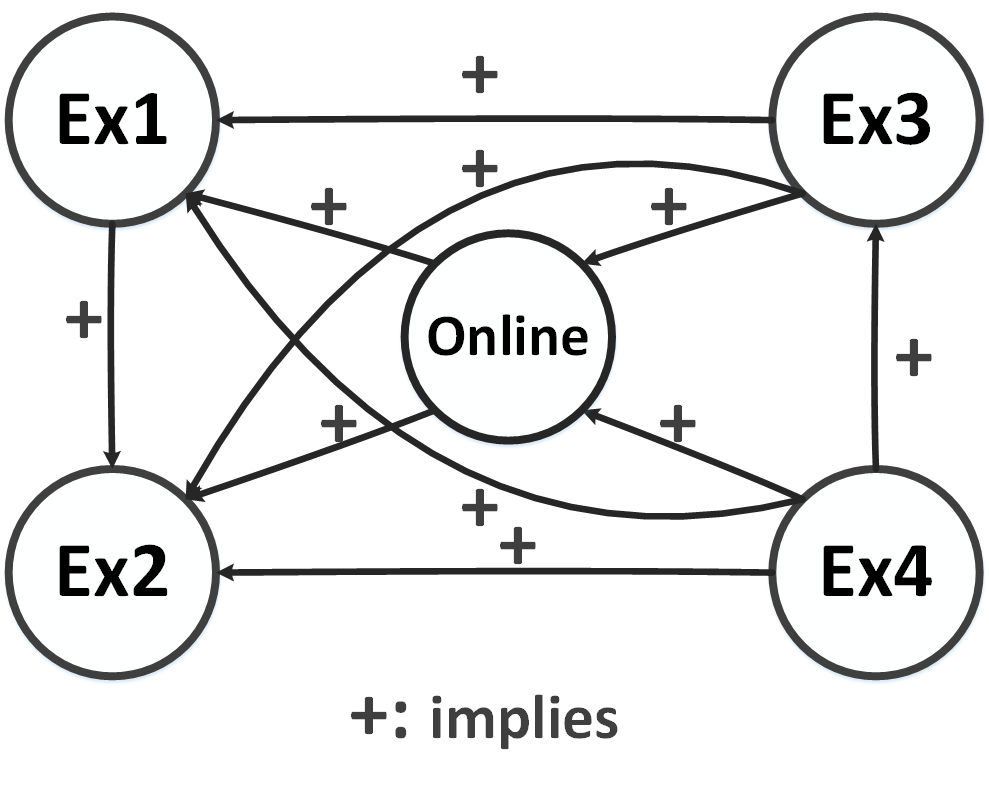
\includegraphics[scale=0.28]{figures/Fig8.png}}
	}}
      
      \caption{The implication relationships graph between existing observability 1, 2, 3, 4, and online observability where ``$\rightarrow$" means ``implies".}
      \label{fig:7}
   \end{figure}

From the implication relationships between online observability and existing observability we know that the online observability can help us solve some problem which can not be solved by existing observability. 
 \begin{itemize}
 \item Firstly, if the systems described by \BCNs\ are online observable but not satisfy the existing third and fourth observability, then the online observability can help us determine their initial state in real time. 
 \item Secondly, it takes least observation costs for us to determine the initial state of some systems described in real time by \BCNs. There are some biological systems depicted by \BCNs, such as the immune systems which can be depicted as the \BCN\ T-cell receptor kinetics model \cite{Klamt2006A}. And there exist input-nodes and state-nodes in this model, for the purpose of obtain the initial state of this \BCN, we must select some state-nodes to be observe at first. However, if we use the online observability of \BCNs\ to determine the initial state of the \BCN\ T-cell receptor kinetics model in real time., then we need least observation costs. 
 \end{itemize}

What is more, with the online observability, we can make some optimizations in the process of determining the initial state. We will represent them in the {\em Section \ref{sec:app}}.
   
   
%When I learned the four existing kinds of observability of \BCNs, I found that if we want to determine the initial state of a \BCN\ by first kind of observability, we need to guess the initial state of the \BCN\ and then check it by its corresponding input sequence. If the initial state we guess is right then we can determine the initial state of this \BCN. But if what we guess is incorrect, we need to guess the initial state again and use its corresponding input sequence to determine the initial state of this \BCN. We repeat this process untll we determine the initial state of this \BCN. But if we can not repeat this process, we can not determine the initial state of the \BCN\ too. Then I turned my gaze to the third observability, this kind of observability makes we can determine the initial state without presupposing the initial state. But I thought if we can determine the possible states set of the \BCN\ by observing the output at first, why do not we find corresponding input sequences for these possible states sets when we determine the initial state of \BCN? Compared with the existing third observability this method needs weaker preconditions of \BCNs\ for us to determine their initial state. Then I talked about this thinkness with my teacher, and we expand it into the original idea of the online observability of \BCNs. 
%==============================================================================================================